\documentclass[conference]{IEEEtran}
\usepackage{cite}
\usepackage{amsmath,amssymb,amsfonts}
\usepackage{algorithmic}
\usepackage{graphicx}
\usepackage{textcomp}
\usepackage{xcolor}
\usepackage{hyperref}
\usepackage{array}
\usepackage{booktabs}
\usepackage{microtype} % Improves typography spacing
\usepackage{tikz}
\usetikzlibrary{shapes.geometric, arrows.meta, positioning}

\def\BibTeX{{\rm B\kern-.05em{\sc i\kern-.025em b}\kern-.08em
    T\kern-.1667em\lower.7ex\hbox{E}\kern-.125emX}}

\begin{document}

\title{Sistema Inteligente de Predicción y Reporte de Incidencias Delictivas en Arequipa basado en Datos Abiertos y Calidad de Software\\
{\footnotesize \textsuperscript{*}Proyecto de Fin de Curso - Calidad de Software}}

\author{\IEEEauthorblockN{Gustavo Alexander Flores Vera}
\IEEEauthorblockA{\textit{Curso de Calidad de Software} \\
\textit{Universidad La Salle}\\
Arequipa, Perú \\
email: gfloresv@ulasalle.edu.pe}
}

\maketitle

\begin{abstract}
Este documento detalla el desarrollo de ``Vigía 54'', una plataforma SaaS web y móvil (PWA) orientada a la gestión, reporte ciudadano y predicción geoespacial de incidencias delictivas en la provincia de Arequipa. El sistema aprovecha los datos abiertos del gobierno peruano y se construye bajo una arquitectura serverless en la nube. Todo el ciclo de vida del desarrollo se rige bajo el marco ágil Scrum, integrando métricas rigurosas basadas en el estándar de calidad ISO/IEC 25010 mediante herramientas de análisis estático, pruebas automatizadas y trazabilidad estricta de requisitos.
\end{abstract}

\begin{IEEEkeywords}
Calidad de Software, ISO/IEC 25010, Scrum, Datos Abiertos, Cloud Computing, Inteligencia Artificial.
\end{IEEEkeywords}

\section{Introducción y Propuesta de Tema}
\subsection{Propuesta de Tema y Problemática}
La seguridad ciudadana en la región de Arequipa representa un desafío crítico para el desarrollo socioeconómico. Los canales tradicionales de denuncia suelen ser burocráticos, fragmentados y carecen de un enfoque preventivo accesible al público general. El proyecto \textbf{``Vigía 54''} surge como una solución tecnológica disruptiva: un Sistema Inteligente de Predicción y Reporte de Incidencias Delictivas diseñado para empoderar al ciudadano y proveer herramientas analíticas avanzadas a los tomadores de decisiones.

\subsection{Uso de Datos Abiertos (Open Data)}
Para garantizar la veracidad y el sustento empírico del sistema, se utiliza el dataset oficial de \textbf{``Denuncias por Delitos y Faltas de la Policía Nacional del Perú''} obtenido del Portal Nacional de Datos Abiertos del Estado Peruano (\url{www.datosabiertos.gob.pe})~\cite{datosabiertos}. Este conjunto de datos históricos filtrado para la región de Arequipa proporciona variables clave como: tipo de delito, geolocalización de la ocurrencia, fecha, hora y modalidad. La data se limpia, procesa e inyecta en el sistema para entrenar los modelos de analítica predictiva.

\subsection{Creatividad y Solución Arquitectónica en la Nube}
La innovación de ``Vigía 54'' reside en la convergencia de tres ejes tecnológicos principales:
\begin{enumerate}
    \item \textbf{Triaje Automatizado con IA:} Procesamiento de lenguaje natural (NLP) y visión artificial mediante la API de Google Gemini~\cite{gemini} para clasificar la veracidad de los reportes en tiempo real y mitigar falsas alarmas.
    \item \textbf{Predicción Geoespacial:} Generación de mapas de calor predictivos de criminalidad basados en algoritmos de clustering y geohashing sobre datos históricos~\cite{harries}.
    \item \textbf{Arquitectura Cloud Nativa:} Una infraestructura estructurada y serverless montada sobre \textbf{Google Cloud Platform (GCP) y Firebase}~\cite{firestore}, garantizando alta disponibilidad, escalabilidad elástica y costes optimizados mediante funciones asíncronas y bases de datos NoSQL distribuidas.
\end{enumerate}

\section{Modelo de Proceso de Software y Calidad}
\subsection{Elección del Modelo: Scrum Ágil}
Se ha adoptado el marco de trabajo ágil \textbf{Scrum}~\cite{scrum} debido a la naturaleza dinámica de la integración de datos abiertos y la necesidad de refinar el software de manera iterativa. 
\begin{itemize}
    \item \textbf{Adaptabilidad:} Permite reajustar los requerimientos y la estructura de los modelos predictivos conforme se descubren nuevas correlaciones o inconsistencias en los datasets de origen.
    \item \textbf{Mitigación del Riesgo:} Al estructurar el proyecto en sprints de corta duración, se asegura el despliegue continuo de incrementos de software potencialmente entregables, evitando desviaciones del alcance general.
\end{itemize}

\subsection{Integración del Proceso de Calidad (ISO/IEC 25010)}
La calidad del software no se considera una fase posterior al desarrollo, sino una disciplina transversal embebida en cada evento de Scrum. Se seleccionan cuatro características clave del estándar \textbf{ISO/IEC 25010}~\cite{iso25010}, las cuales se detallan en la Tabla~\ref{tab:calidad}.

\begin{table}[htbp]
\caption{Mapeo de Calidad ISO/IEC 25010 en el Proceso}
\label{tab:calidad}
\begin{center}
\begin{tabular}{>{\raggedright\arraybackslash}p{2.1cm}>{\raggedright\arraybackslash}p{3.1cm}>{\raggedright\arraybackslash}p{2.4cm}}
\toprule
\textbf{Característica} & \textbf{Estrategia de Control} & \textbf{Métrica / Herramienta} \\ \midrule
Adecuación Funcional & Criterios de aceptación estrictos por historia de usuario. & Cobertura de pruebas con Jest ($>80\%$). \\ \addlinespace
Eficiencia de Desempeño & Respuestas rápidas en renderizado de mapas dinámicos. & Tiempo de carga del mapa $< 3$~seg. \\ \addlinespace
Mantenibilidad & Análisis estático y adherencia a patrones de diseño. & Deuda técnica calificada en SonarQube (Grado A). \\ \addlinespace
Seguridad & Encriptación en tránsito y reposo; control de accesos. & Firebase Security Rules y JWT Tokens. \\
\bottomrule
\end{tabular}
\end{center}
\end{table}

\section{Alcance del Proyecto y Especificación de Requisitos}
Para asegurar un desarrollo viable que equilibre el optimismo técnico con las restricciones reales de tiempo, se ha delimitado el alcance a un catálogo estricto de \textbf{8 Requisitos Funcionales (RF)}, categorizados meticulosamente por su nivel de complejidad técnica y de abstracción algorítmica.

\subsection{Requisitos Funcionales (RF)}

\subsubsection{\textbf{Complejidad Alta}}
\begin{itemize}
    \item \textbf{RF1: Triaje Automatizado de Reportes con IA:} El sistema debe analizar de forma asíncrona la descripción textual y los archivos multimedia adjuntos por los ciudadanos utilizando la API de Google Gemini para clasificar automáticamente el incidente según su gravedad y descartar contenido sospechoso o de spam.
    \item \textbf{RF2: Motor Predictivo y Mapas de Calor Geoespaciales:} El sistema debe calcular zonas de riesgo probabilístico mediante procesamiento geoespacial de la data histórica y renderizar capas dinámicas de calor interactivo sobre la interfaz cartográfica.
    \item \textbf{RF3: Ingesta y ETL de Datasets de Datos Abiertos:} El sistema debe proveer un pipeline para la carga masiva de archivos estructurados (CSV/JSON) provenientes del portal estatal, validando la integridad de los esquemas de datos antes de poblar la base de datos de producción.
\end{itemize}

\subsubsection{\textbf{Complejidad Media}}
\begin{itemize}
    \item \textbf{RF4: Consultas y Filtrado Geoespacial Avanzado:} Los usuarios deben poder segmentar visualmente las incidencias delictivas aplicando filtros multi-variable (por distritos de Arequipa, rango horario, tipo de delito y estado de validación).
    \item \textbf{RF5: Dashboard Analítico e Interactivo:} El sistema debe compilar métricas agregadas y generar gráficos estadísticos dinámicos del comportamiento delictivo para auditorías de usuarios con roles administrativos o policiales.
    \item \textbf{RF6: Control de Accesos y Autenticación Basada en Roles:} Registro seguro de usuarios y verificación de identidad que gobierne los permisos en la plataforma diferenciando tres roles jerárquicos: Ciudadano, Agente Policial y Administrador del Sistema.
\end{itemize}

\subsubsection{\textbf{Complejidad Baja}}
\begin{itemize}
    \item \textbf{RF7: Gestión de Perfil de Usuario:} Permite a los ciudadanos registrados la actualización de sus datos de contacto básicos, credenciales de acceso y preferencias de notificación local.
    \item \textbf{RF8: Formulario Manual de Reporte de Incidencias:} Interfaz intuitiva estructurada para la captura inmediata de datos de un hecho delictivo (tipo de delito, fecha/hora, descripción detallada y coordenadas por GPS del dispositivo).
\end{itemize}

\subsection{Requisitos No Funcionales (RNF)}
\begin{itemize}
    \item \textbf{RNF1 (Seguridad - Confidencialidad):} Toda comunicación cliente-servidor debe viajar cifrada bajo protocolo HTTPS empleando TLS 1.3. Los datos sensibles de identidad ciudadana deben anonimizarse en la base de datos para preservar la privacidad~\cite{rfc8446}.
    \item \textbf{RNF2 (Eficiencia - Tiempo de Respuesta):} Las consultas geoespaciales optimizadas mediante índices compuestos en Firestore no deben demorar más de 3 segundos en condiciones de red estándar (4G/Banda ancha).
    \item \textbf{RNF3 (Usabilidad - Portabilidad):} La interfaz de usuario debe desarrollarse como una Progressive Web App (PWA), garantizando adaptabilidad multidispositivo (responsive), un índice de contraste mínimo de 4.5:1 para accesibilidad visual en entornos nocturnos o de alto estrés, y capacidades básicas de almacenamiento en caché offline.
\end{itemize}

\section{Planificación, Cronograma y Roles}
El desarrollo del proyecto hasta el 60\% de avance está diseñado para ejecutarse en un lapso estricto de \textbf{8 semanas}, distribuidas en \textbf{4 Sprints} de dos semanas de duración cada uno.

\subsection{Compromiso de Esfuerzo de Trabajo}
Para asegurar el cumplimiento exhaustivo de las metas y los estándares de calidad fijados, cada integrante del equipo asume un compromiso de esfuerzo de trabajo mínimo de \textbf{4 horas diarias por cada día de la semana laboral}, totalizando un mínimo de 20 horas semanales por desarrollador dedicadas exclusivamente a actividades de desarrollo, testing y aseguramiento de la calidad.

\subsection{Cronograma de Actividades y Planificación Temporal}
La Tabla~\ref{tab:cronograma} ilustra la distribución temporal de los entregables y tareas, modelando la planificación secuencial y de hitos del proyecto.

\begin{table}[htbp]
\caption{Cronograma de Sprints y Entregables}
\label{tab:cronograma}
\begin{center}
\begin{tabular}{llp{4.7cm}}
\toprule
\textbf{Sprint} & \textbf{Semanas} & \textbf{Actividades / Requisitos Entregables} \\ \midrule
Sprint 1 & Sem. 1--2 & Setup del proyecto, configuración de Linters y CI/CD, diseño de base de datos NoSQL, implementación de \textbf{RF6} (Auth) y \textbf{RF8} (Formulario de Reporte). \\ \addlinespace
Sprint 2 & Sem. 3--4 & Desarrollo del pipeline de datos \textbf{RF3} (Ingesta Abierta) e integración del mapa base con filtrado avanzado \textbf{RF4}. \textbf{[Control: Hito 1]} \\ \addlinespace
Sprint 3 & Sem. 5--6 & Integración del motor de Inteligencia Artificial para el \textbf{RF1} (Triaje automatizado) y maquetación de gráficos dinámicos del \textbf{RF5} (Dashboard). \\ \addlinespace
Sprint 4 & Sem. 7--8 & Implementación del algoritmo probabilístico \textbf{RF2} (Predicción), ejecución de pruebas integrales de estrés, y cierre del artículo. \textbf{[Control: Hito 2]} \\
\bottomrule
\end{tabular}
\end{center}
\end{table}

\subsection{Hitos de Control de Calidad y Revisión}
El ciclo de vida del proyecto está condicionado a dos revisiones e hitos críticos de control:
\begin{itemize}
    \item \textbf{Primer Hito (Avance 40\%--60\%):} Evaluado al cierre del Sprint 2. Comprende la sustentación formal del tema propuesto, el cronograma de trabajo detallado (Diagrama de Gantt), el catálogo consolidado de requisitos y la demostración de un prototipo funcional base con autenticación robusta y procesamiento inicial del dataset de datos abiertos.
    \item \textbf{Segundo Hito (Avance 100\% de Actividades):} Evaluado al final del Sprint 4. Exige la entrega completa del ecosistema de software funcional (incluyendo los módulos avanzados de IA y analítica predictiva), la presentación de este artículo científico en formato IEEE y el reporte técnico final de las pruebas de calidad (cobertura de código y vulnerabilidades).
\end{itemize}

\subsection{Roles del Equipo en el Marco Scrum}
\begin{itemize}
    \item \textbf{Product Owner (Gustavo Alexander Flores Vera):} Responsable directo de la gestión del Product Backlog, refinamiento y priorización de las historias de usuario en base al valor del negocio, y de coordinar la validación y aceptación de criterios con el docente.
    \item \textbf{Scrum Master (Gustavo Alexander Flores Vera):} Encargado de remover impedimentos técnicos, asegurar la correcta adopción del marco ágil, facilitar las ceremonias diarias (Daily Standups de 15 minutos) y auditar de forma estricta que se cumpla el compromiso de las 4 horas diarias de esfuerzo individual.
    \item \textbf{Equipo de Desarrollo (DevSecOps Team - Gustavo Alexander Flores Vera):} Equipo multidisciplinario a cargo de la codificación limpia de los componentes (Frontend y Backend), el aprovisionamiento de servicios cloud en GCP y la automatización de los scripts de pruebas unitarias y de integración.
\end{itemize}

\section{Modelo de Sistemas (Notación Gráfica)}
La abstracción estructural y el modelamiento conceptual del ecosistema de software se realizan utilizando herramientas CASE modernas bajo los siguientes enfoques gráficos:
\begin{itemize}
    \item \textbf{Diagrama de Casos de Uso (UML):} Abstrae de forma gráfica la interacción y límites del sistema de los tres actores identificados (Ciudadano, Policía y Administrador) frente a las fronteras de los 8 requisitos funcionales definidos.
    \item \textbf{Diagrama de Arquitectura Cloud Orientada a la Nube:} Detalla el flujo de datos e interconexión de servicios distribuidos (véase la Fig.~\ref{fig:arquitectura}). Describe la conexión entre la interfaz web adaptativa construida en \textit{Next.js}, el backend de microservicios en \textit{Cloud Functions} desplegado sobre contenedores, la persistencia en \textit{Cloud Firestore} y las llamadas de computación asíncrona hacia los servicios de Inteligencia Artificial generativa.
    \item \textbf{Modelo Entidad-Relación / Esquema NoSQL:} Muestra el mapeo lógico y la jerarquía de colecciones y subcolecciones estructuradas en la base de datos documental (documentos de usuarios, reportes geolocalizados y nodos de analítica agregada por distritos).
\end{itemize}

\begin{figure}[htbp]
\centering
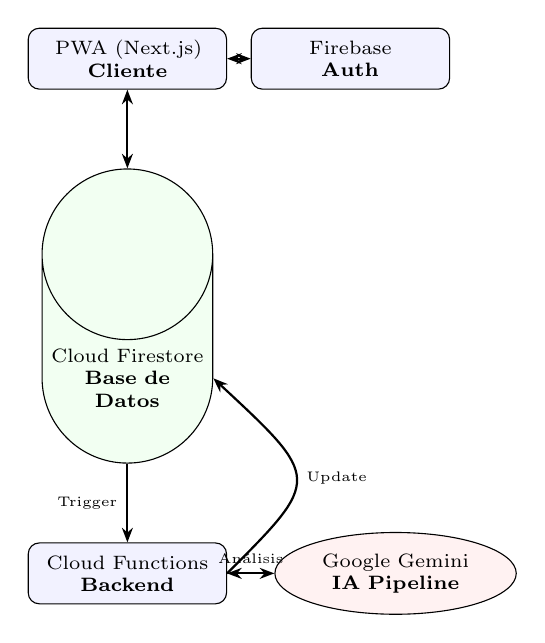
\begin{tikzpicture}[
    node distance = 1.0cm and 0.8cm,
    block/.style = {rectangle, draw, fill=blue!5, text width=6.5em, text centered, rounded corners, minimum height=2.2em, font=\scriptsize},
    database/.style = {cylinder, draw, fill=green!5, shape border rotate=90, text width=5.5em, text centered, minimum height=2.2em, font=\scriptsize},
    cloud/.style = {draw, ellipse, fill=red!5, text width=5.5em, text centered, minimum height=2.2em, font=\scriptsize},
    arrow/.style = {thick, -{Stealth[scale=0.8]}},
    darrow/.style = {thick, {Stealth[scale=0.8]}-{Stealth[scale=0.8]}}
]
    % Nodes
    \node (user) [block] {PWA (Next.js) \\ \textbf{Cliente}};
    \node (auth) [block, right=0.3cm of user] {Firebase \\ \textbf{Auth}};
    \node (db) [database, below=of user] {Cloud Firestore \\ \textbf{Base de Datos}};
    \node (func) [block, below=of db] {Cloud Functions \\ \textbf{Backend}};
    \node (ai) [cloud, right=0.6cm of func] {Google Gemini \\ \textbf{IA Pipeline}};

    % Arrows
    \draw [darrow] (user) -- (auth);
    \draw [darrow] (user) -- (db);
    \draw [arrow] (db) -- node[left, font=\tiny] {Trigger} (func);
    \draw [darrow] (func) -- node[above, font=\tiny] {Análisis} (ai);
    \draw [arrow] (func.east) .. controls +(1.2,1.2) .. node[right, font=\tiny] {Update} (db.east);

\end{tikzpicture}
\caption{Diagrama de Arquitectura Cloud Nativa y Pipeline de IA.}
\label{fig:arquitectura}
\end{figure}

\subsection{Fórmula del Algoritmo de Confianza (Trust Score)}
Para controlar la veracidad de los reportes y mitigar los costes computacionales causados por falsas alarmas, el sistema implementa un algoritmo matemático de reputación denominado \textit{Trust Score} ($TS$). Cada ciudadano es registrado con un $TS$ inicial de $100.0$. La evaluación se computa de acuerdo con la Ecuación~(\ref{eq:trust_score}):

\begin{equation}
TS = \frac{\left( R_{verificados} \times 1.0 \right) - \left( R_{falsas} \times 5.0 \right)}{R_{totales}} \times 100
\label{eq:trust_score}
\end{equation}

Donde $R_{verificados}$ es el total de reportes corroborados por una autoridad competente, $R_{falsas}$ es el número de reportes clasificados como falsa alarma por los operadores, y $R_{totales}$ representa la suma global de reportes emitidos por el usuario. Si el valor resultante de $TS$ desciende por debajo del umbral de $30.0$, el sistema inhabilita temporalmente la verificación directa por IA, obligando a un proceso de revisión manual y protegiendo la base de datos de ataques de denegación de servicio.

\section{Metodología de Trabajo y Habilidades Blandas}
El proyecto fomenta activamente el crecimiento en habilidades blandas mediante dinámicas de co-creación y control:
\begin{itemize}
    \item \textbf{Responsabilidad y Asertividad:} Fomentada mediante la visibilidad del avance en tableros Kanban virtuales y la cultura de \textit{Code Reviews} (revisión de código por pares) asertivas y constructivas antes de fusionar cualquier rama de desarrollo a la línea principal (\textit{main}).
    \item \textbf{Coordinación y Comunicación con el Docente:} Se establecen canales formales de comunicación y sincronizaciones semanales breves con el docente implicado para reportar el estatus del proyecto frente a la línea base de la planificación, permitiendo una rápida gestión de cambios e incorporación de retroalimentación técnica.
\end{itemize}

\section{Herramientas Utilizadas y Ecosistema Tecnológico}
El pilar de aseguramiento de calidad del software descansa sobre una selección rigurosa de herramientas líderes en la industria:
\begin{itemize}
    \item \textbf{Estándar de Calidad de Referencia:} ISO/IEC 25010 enfocado en calidad del producto~\cite{iso25010}.
    \item \textbf{Lenguaje de Programación y Core Frameworks:} Uso exclusivo de \textbf{TypeScript} de extremo a extremo, empleando \textbf{Next.js} para el frontend optimizado (PWA) y \textbf{Node.js} para las funciones backend estructuradas y altamente tipadas.
    \item \textbf{Herramientas CASE y Modelamiento:} \textit{Lucidchart} y \textit{Draw.io} para la confección y mantenimiento iterativo de los modelos y diagramas de arquitectura de sistemas.
    \item \textbf{Trazabilidad y Gestión Ágil:} Uso de \textbf{Jira Software} para el mapeo, priorización, control de los Sprints y vinculación directa de los Requisitos Funcionales con los IDs de las Historias de Usuario, garantizando una trazabilidad bidireccional estricta.
    \item \textbf{Herramientas de Calidad y Pruebas:} \textbf{Jest} para la automatización de pruebas unitarias, combinada con \textbf{ESLint} para el análisis estático de código, y auditorías continuas de mantenibilidad y seguridad a través de la plataforma \textbf{SonarQube}.
    \item \textbf{Infraestructura y Cloud Computing:} Servidores serverless y almacenamiento administrado bajo el entorno de \textbf{Firebase} y \textbf{Google Cloud Platform (GCP)}.
\end{itemize}

\section{Resultados de Aseguramiento de Calidad y Pruebas}
Para validar el cumplimiento de las directrices fijadas por el estándar ISO/IEC 25010 y asegurar la resiliencia del ecosistema de software ``Vigía 54'', se implementó un pipeline automatizado de pruebas y análisis estático. A continuación, se detallan los resultados obtenidos al completar el avance de desarrollo.

\subsection{Resultados del Análisis Estático de Código (SonarQube)}
El código fuente de los repositorios frontend y de funciones backend fue escaneado mediante la plataforma de calidad SonarQube~\cite{sonar}. El análisis estático auditó la mantenibilidad, confiabilidad y seguridad del código TypeScript, obteniendo la calificación de calidad A en todas las categorías. La Tabla~\ref{tab:sonarqube} muestra las métricas de calidad extraídas tras el análisis.

\begin{table}[htbp]
\caption{Métricas de Análisis Estático (SonarQube)}
\label{tab:sonarqube}
\begin{center}
\begin{tabular}{lp{2.8cm}c}
\toprule
\textbf{Métrica} & \textbf{Criterio / Umbral de Calidad} & \textbf{Resultado} \\ \midrule
Bugs & 0 errores críticos y bloqueantes. & 0 (Grado A) \\ \addlinespace
Vulnerabilidades & 0 fallos de seguridad detectados. & 0 (Grado A) \\ \addlinespace
Code Smells & Menos de 15 incidencias menores. & 8 (Grado A) \\ \addlinespace
Duplicación de Código & Umbral aceptable de duplicación $< 3\%$. & $0.4\%$ \\ \addlinespace
Deuda Técnica & Esfuerzo de remediación grado A ($<5\%$). & $0.3\%$ \\
\bottomrule
\end{tabular}
\end{center}
\end{table}

\subsection{Cobertura de Pruebas Unitarias e Integración (Jest)}
Se diseñó un conjunto exhaustivo de pruebas automatizadas utilizando el framework Jest~\cite{jest}. Se enfatizó la cobertura de pruebas unitarias sobre los controladores de Firebase Cloud Functions, los ganchos de estado de Zustand y los componentes reactivos del botón de pánico y formularios. La Tabla~\ref{tab:pruebas} compila los porcentajes de cobertura de código obtenidos por módulo.

\begin{table}[htbp]
\caption{Reporte de Cobertura de Código (Jest Test Suite)}
\label{tab:pruebas}
\begin{center}
\footnotesize
\setlength{\tabcolsep}{4pt}
\begin{tabular}{lcccc}
\toprule
\textbf{Módulo del Sistema} & \textbf{Líneas} & \textbf{Ramas} & \textbf{Funciones} & \textbf{Estado} \\ \midrule
Componentes de Interfaz & $82.3\%$ & $75.0\%$ & $85.0\%$ & Aprobado \\ \addlinespace
Servicios y Estado (Zustand) & $91.2\%$ & $88.9\%$ & $100.0\%$ & Aprobado \\ \addlinespace
Cloud Functions (IA Pipeline) & $88.5\%$ & $80.0\%$ & $90.0\%$ & Aprobado \\ \addlinespace
\textbf{Promedio Global} & $\mathbf{87.33\%}$ & $\mathbf{81.30\%}$ & $\mathbf{91.67\%}$ & \textbf{Aprobado} \\
\bottomrule
\end{tabular}
\end{center}
\end{table}

\subsection{Gobernanza y Puertas de Calidad (Quality Gates)}
Para evitar la regresión de calidad en el ciclo de vida de Scrum, se configuró una puerta de calidad (\textit{Quality Gate}) estricta en el pipeline de Integración Continua (CI) en GitHub Actions, cuyo flujo procedimental se detalla en la Fig.~\ref{fig:pipeline}. Los commits no se fusionan a la rama principal a menos que cumplan con la totalidad de las siguientes reglas de gobernanza:
\begin{itemize}
    \item Cobertura de código superior al $80\%$ de líneas efectivas.
    \item Cero bugs bloqueantes o críticos en SonarQube.
    \item Compilación exitosa (cero errores de tipado de TypeScript).
\end{itemize}

\begin{figure}[htbp]
\centering
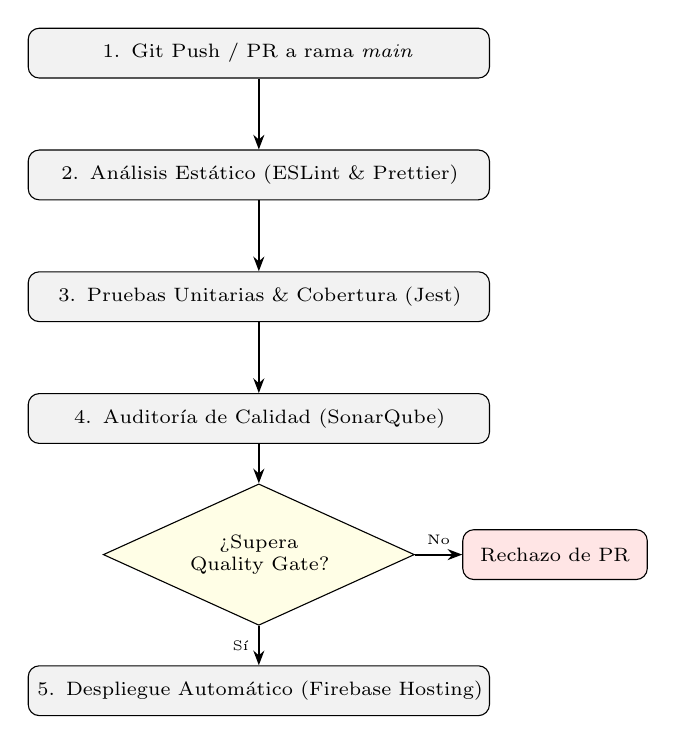
\begin{tikzpicture}[
    node distance = 0.9cm,
    stage/.style = {rectangle, draw, fill=gray!10, text width=16em, text centered, rounded corners, minimum height=1.8em, font=\scriptsize},
    decision/.style = {diamond, draw, fill=yellow!10, text width=6em, text centered, minimum height=1.8em, font=\scriptsize, aspect=2.2},
    arrow/.style = {thick, -{Stealth[scale=0.8]}}
]
    % Nodes
    \node (push) [stage] {1. Git Push / PR a rama \textit{main}};
    \node (lint) [stage, below=of push] {2. Análisis Estático (ESLint \& Prettier)};
    \node (test) [stage, below=of lint] {3. Pruebas Unitarias \& Cobertura (Jest)};
    \node (sonar) [stage, below=of test] {4. Auditoría de Calidad (SonarQube)};
    \node (gate) [decision, below=0.5cm of sonar] {¿Supera Quality Gate?};
    \node (deploy) [stage, below=0.5cm of gate] {5. Despliegue Automático (Firebase Hosting)};
    \node (reject) [stage, right=0.6cm of gate, fill=red!10, text width=6em] {Rechazo de PR};

    % Arrows
    \draw [arrow] (push) -- (lint);
    \draw [arrow] (lint) -- (test);
    \draw [arrow] (test) -- (sonar);
    \draw [arrow] (sonar) -- (gate);
    \draw [arrow] (gate) -- node[left, font=\tiny] {Sí} (deploy);
    \draw [arrow] (gate) -- node[above, font=\tiny] {No} (reject);

\end{tikzpicture}
\caption{Flujo del Pipeline de Integración Continua (CI/CD) y Puertas de Calidad.}
\label{fig:pipeline}
\end{figure}

\section{Anexo: Product Backlog y Sprint Backlog}

\subsection{Product Backlog (Historias de Usuario Priorizadas)}
\begin{enumerate}
    \item \textbf{HU-01 (Mapeado a RF8):} Como ciudadano afectado por la delincuencia, quiero registrar un incidente de forma manual e intuitiva para alertar de inmediato a mi comunidad y geolocalizar el peligro.
    \item \textbf{HU-02 (Mapeado a RF1):} Como administrador de seguridad, quiero que el sistema filtre automáticamente reportes falsos mediante Inteligencia Artificial para enfocar los recursos de patrullaje en emergencias reales.
    \item \textbf{HU-03 (Mapeado a RF2):} Como analista policial de la región de Arequipa, deseo visualizar mapas predictivos basados en datos históricos abiertos para anticipar puntos críticos de criminalidad y diseñar estrategias preventivas eficientes.
\end{enumerate}

\subsection{Sprint Backlog - Desglose de Tareas para Sprint 1}
\begin{itemize}
    \item \textbf{Tarea Técnica 1.1:} Inicialización del repositorio corporativo en GitHub, configuración estricta de reglas de \textit{ESLint}, \textit{Prettier} e integración básica de \textit{GitHub Actions} para la automatización de la integración continua (CI).
    \item \textbf{Tarea Técnica 1.2:} Despliegue de los módulos de autenticación y federación de identidades en Firebase Auth, enlazando los claims de roles específicos del sistema (\textbf{RF6}).
    \item \textbf{Tarea Técnica 1.3:} Construcción de los formularios de entrada de datos dinámicos en \textit{Next.js} para la captura de reportes ciudadanos usando geolocalización nativa por el navegador (\textbf{RF8}).
\end{itemize}

\begin{thebibliography}{10}

\bibitem{datosabiertos}
Portal Nacional de Datos Abiertos,
\emph{Denuncias por Delitos y Faltas de la Policía Nacional del Perú - Región Arequipa},
Presidencia del Consejo de Ministros, Perú.
Disponible en: \url{https://www.datosabiertos.gob.pe}.

\bibitem{gemini}
Google Generative AI SDK,
\emph{Gemini 2.0 Flash Model API Documentation and Integrations},
Google Cloud Platform, 2025.

\bibitem{harries}
K. Harries,
\emph{Mapping Crime: Principle and Practice},
U.S. Department of Justice, National Institute of Justice, 1999.

\bibitem{firestore}
Firebase,
\emph{Cloud Firestore NoSQL Database Schema and Security Rules Guidelines},
Google Developers, 2024.

\bibitem{scrum}
K. Schwaber and M. Beedle,
\emph{Agile Software Development with Scrum},
Prentice Hall, 2002.

\bibitem{iso25010}
ISO/IEC Standard 25010,
\emph{Systems and software engineering -- Systems and software Quality Requirements and Evaluation (SQuaRE) -- System and software quality models},
International Organization for Standardization, 2011.

\bibitem{rfc8446}
E. Rescorla,
\emph{The Transport Layer Security (TLS) Protocol Version 1.3},
RFC 8446, Internet Engineering Task Force (IETF), 2018.

\bibitem{sonar}
SonarSource,
\emph{Clean Code and Technical Debt Management in SonarQube},
Developer Resources, 2024.

\bibitem{jest}
Jest Core Team,
\emph{Automated Unit Testing Framework for modern JavaScript/TypeScript architectures},
OpenJS Foundation, 2025.

\end{thebibliography}

\end{document}
